\documentclass[UTF8]{ctexart}
\usepackage{amsmath}
\usepackage{graphicx}
\title{\heiti 引力波作业报告}
\author{\kaishu 刘苏明}
\date{\today}

\begin{document}
\maketitle

当不对数据作任何处理时,我们无法看到任何的引力波信号,因为引力波信号主要以低频形式存在。对源数据进行带通滤波处理,其频带为[35hz,350Hz],这是探测器的有效探测频带。 由于两个探测器相对位置的差异,引力波从LIGO传播到Livingston需要大约6.9ms且数据大小刚好相反。进行这些数据处理后,得到LIGO和Livingston探测到的引力波随时间变化图,如图一所示。
\begin{figure}[h]
\centering
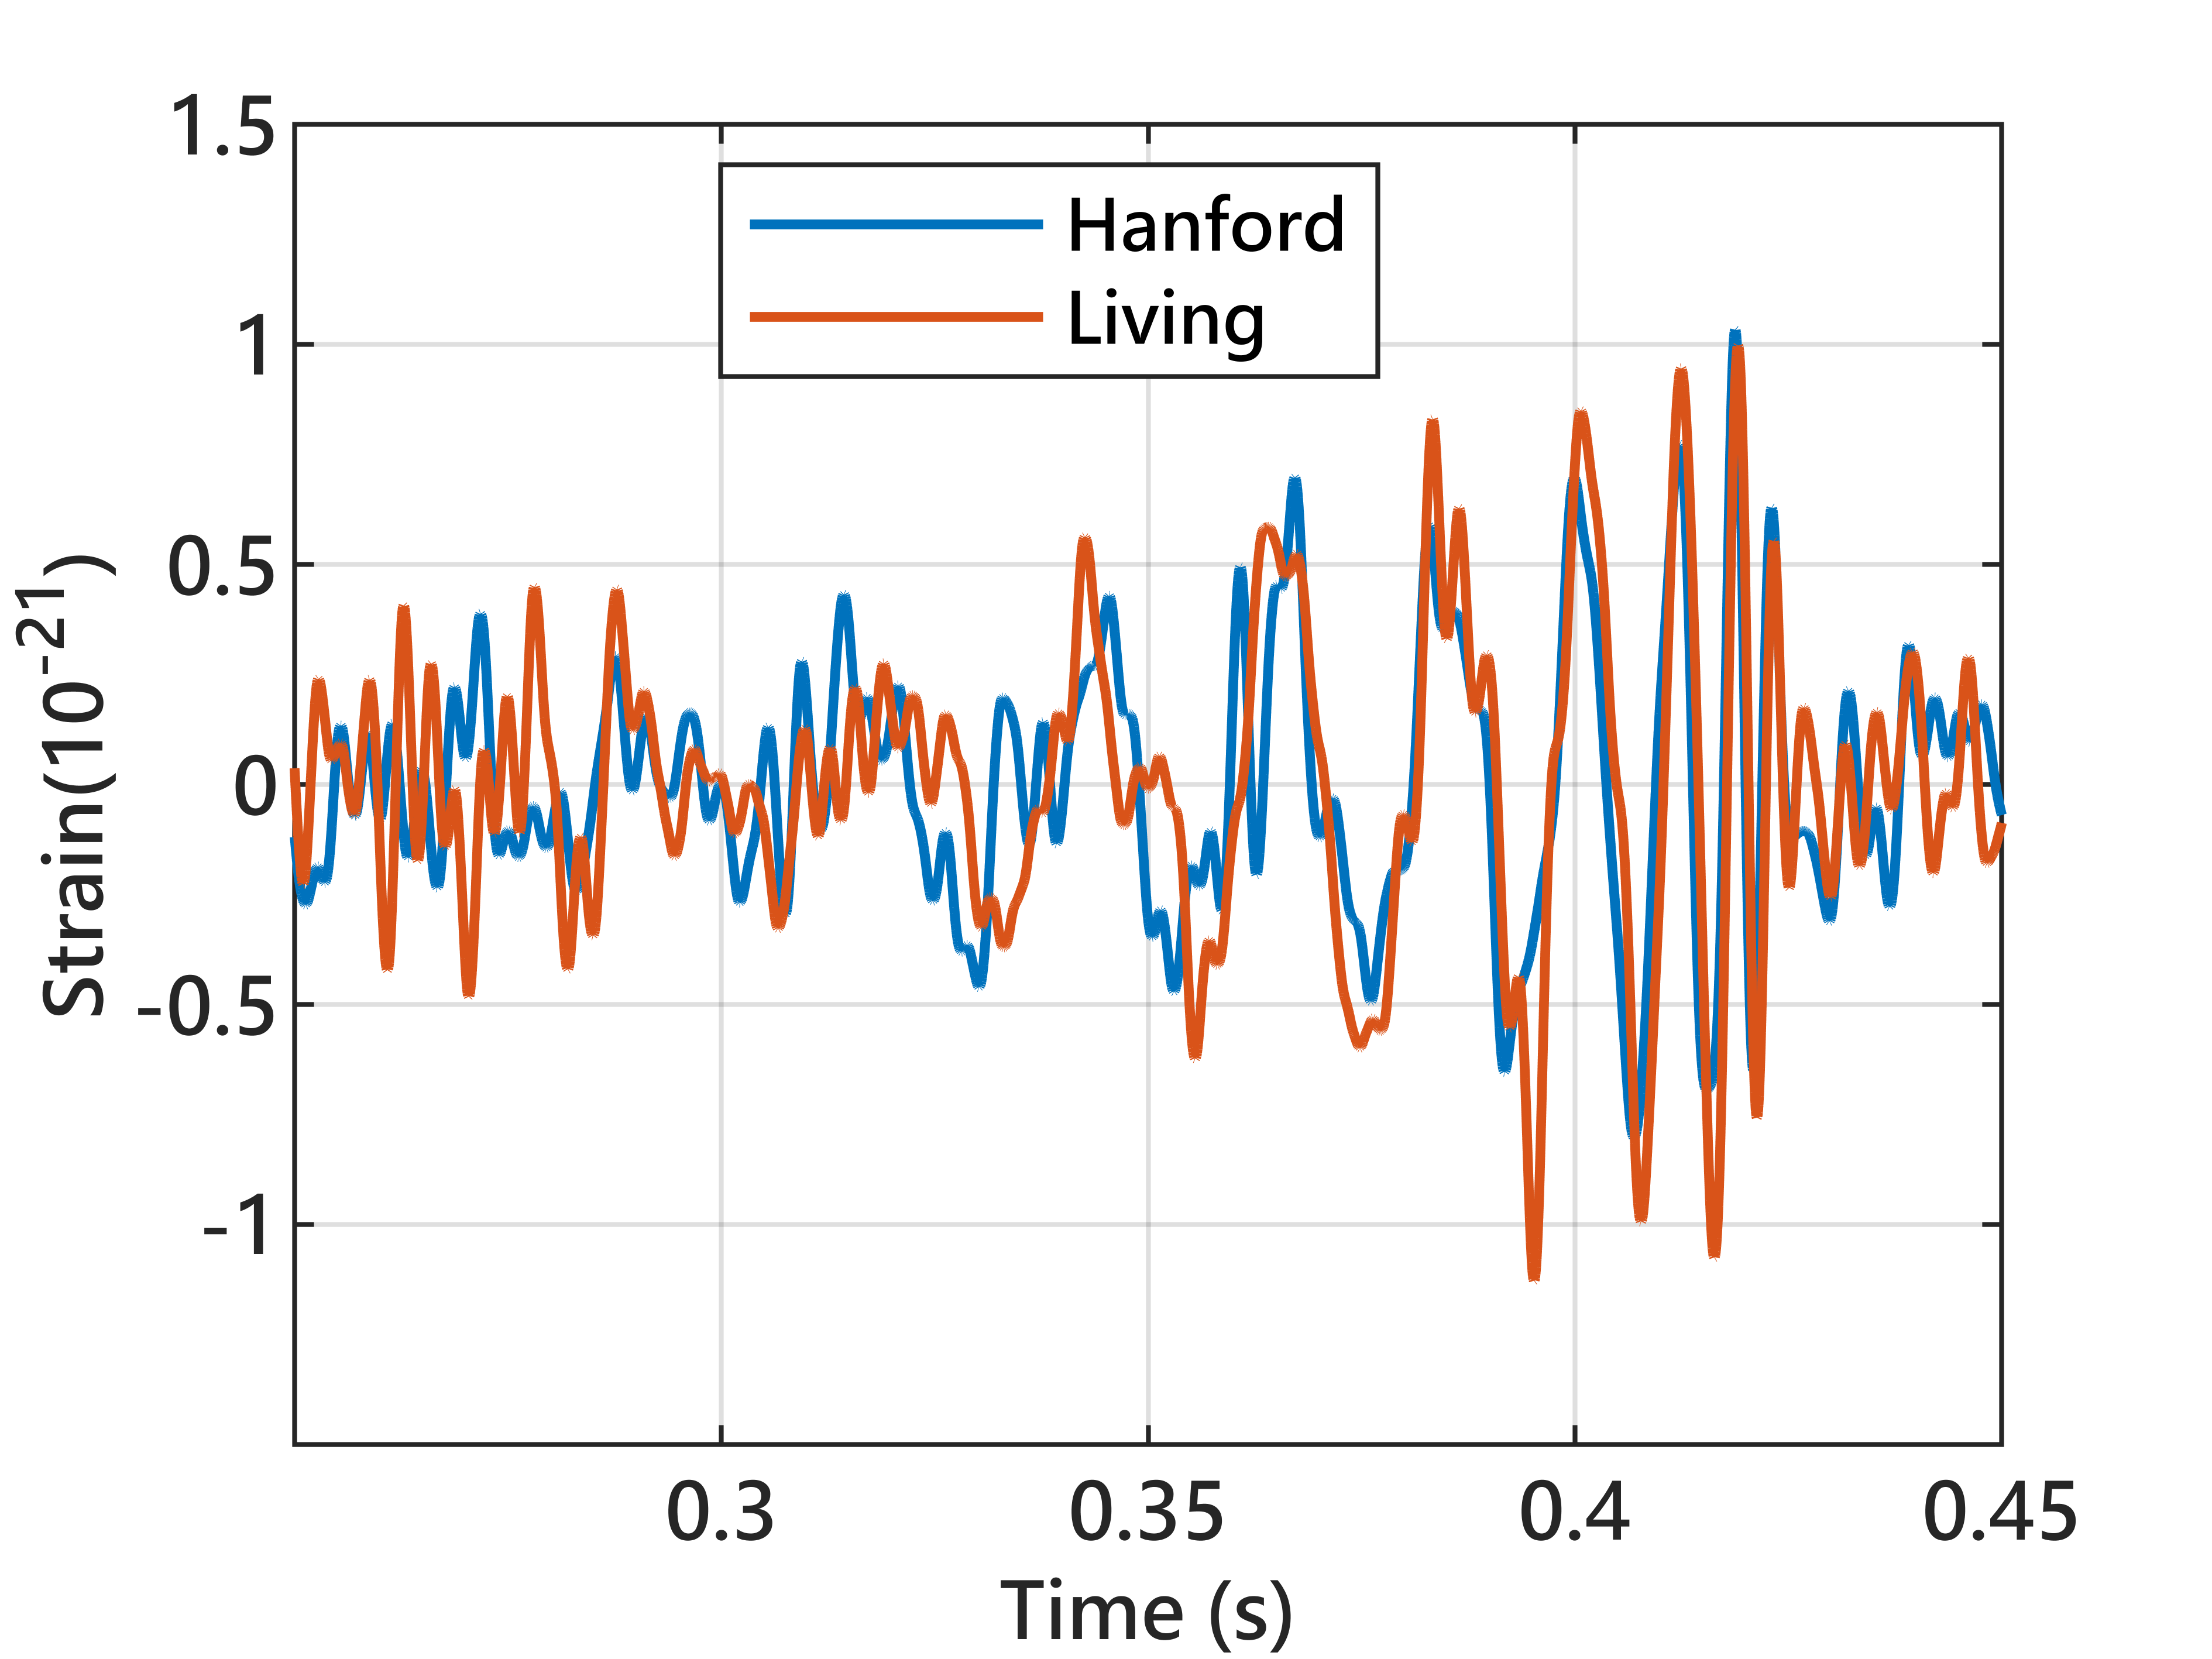
\includegraphics[scale = 0.5]{引力波.png}
\caption{引力波随时间变化}
\end{figure}

图二为引力波信号的时间-频率图。
\begin{figure}[h]
\centering
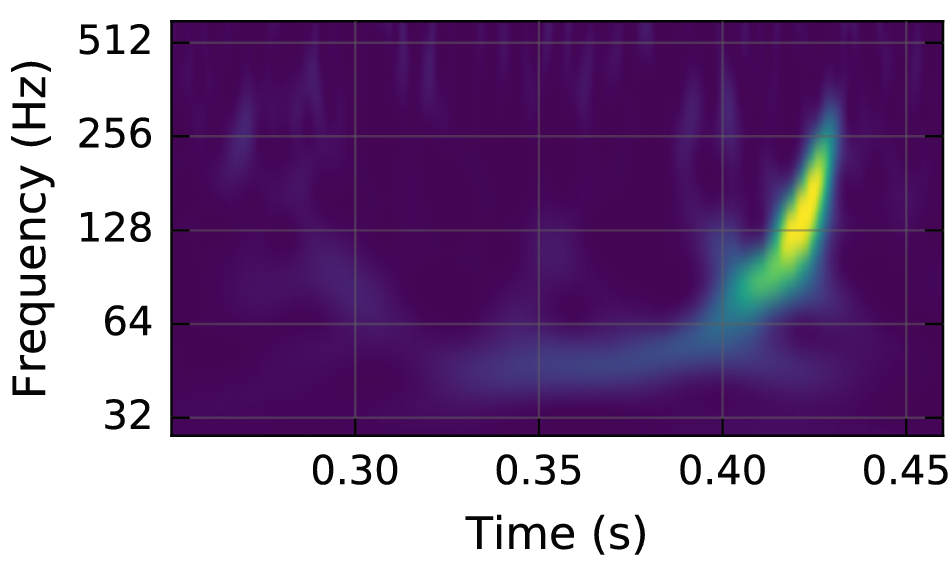
\includegraphics[scale = 0.2]{时频图.png}
\caption{引力波的时频图}
\end{figure}
我们也可以使用过零检测得到$\Delta t$来近似估计时间-频率关系,$f_{GW} = 1/(2\Delta t)$,这样就不用计算引力波模型,简化计算。我们在图三画出近似频率$f_{GW}$的$-8/3$次方


\end{document}